\chapter{Конструкторский раздел}

\section{Описание использованных типов данных}

Для реализации алгоритма использованы:

\begin{itemize}[label=---]
	\item целое число для размерности алфавита;
	\item целое число для количества роторов;
	\item двумерный массив целых чисел для роторов;
	\item одномерный массив целых чисел для коммутационной панели;
	\item одномерный массив целых чисел для рефлектора.
\end{itemize}

\section{Разработка алгоритмов}

На рисунке \ref{img:enigma} представлена схема реализации алгоритма шифрования машины <<Энигма>>.

\begin{table}[H]
	\centering
	\begin{tabular}{p{1\linewidth}}
		\centering
		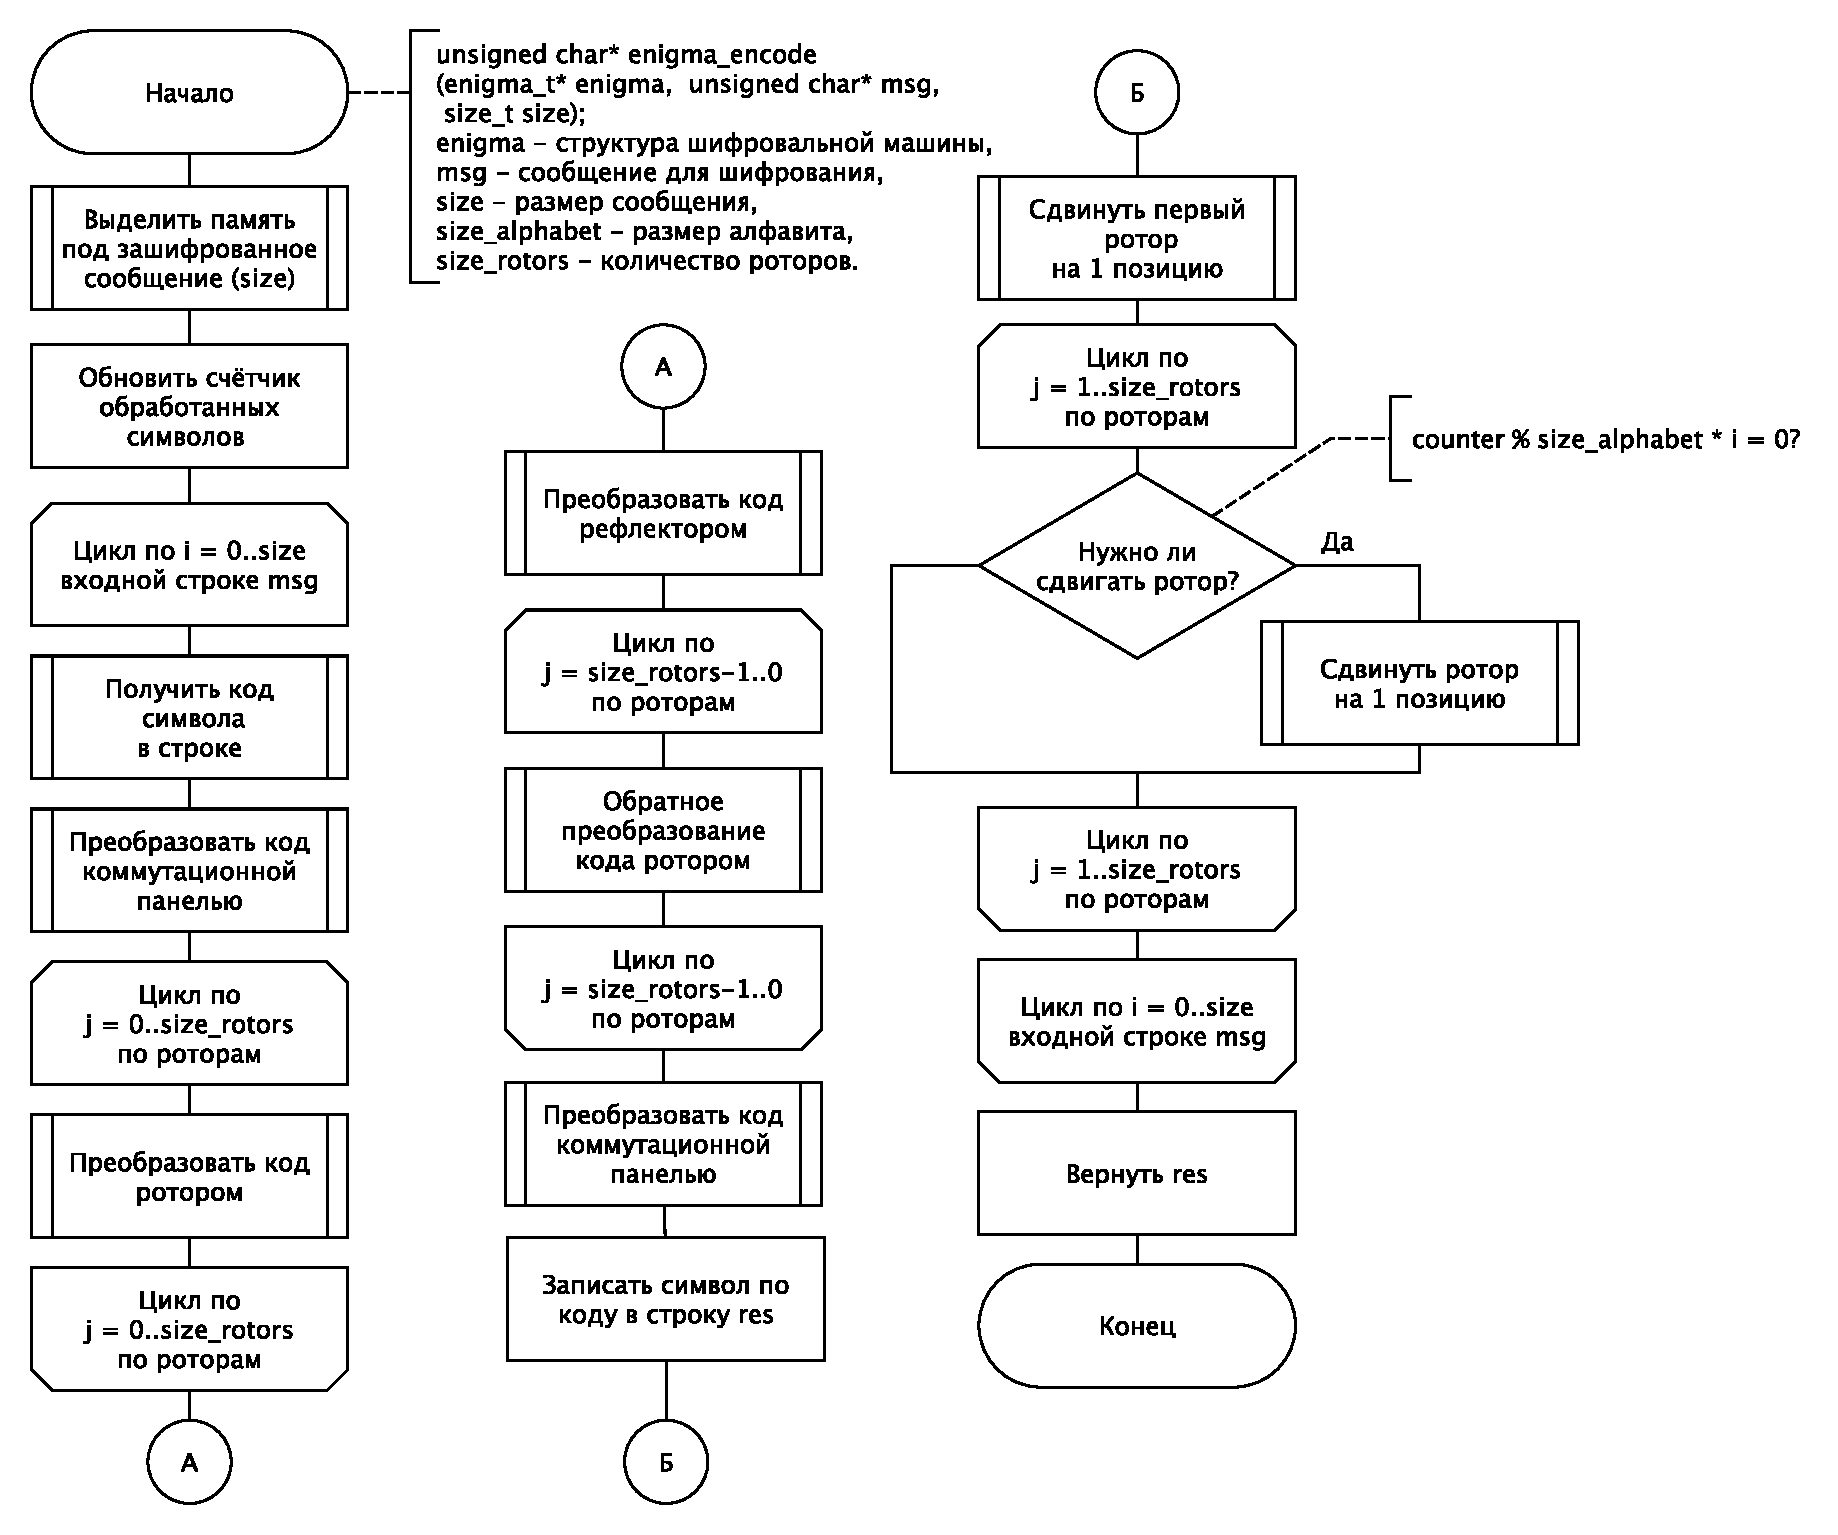
\includegraphics[width=1\linewidth]{inc/pdfs/encode.pdf}
		\captionof{figure}{Схема реализации алгоритма шифрования машины <<Энигма>>}
		\label{img:enigma}
	\end{tabular}
\end{table}
